
\documentclass{article}

\usepackage[preprint]{neurips_2023}
\usepackage[utf8]{inputenc} % allow utf-8 input
\usepackage[T1]{fontenc}    % use 8-bit T1 fonts
\usepackage{hyperref}       % hyperlinks
\usepackage{url}            % simple URL typesetting
\usepackage{booktabs}       % professional-quality tables
\usepackage{amsfonts}       % blackboard math symbols
\usepackage{nicefrac}       % compact symbols for 1/2, etc.
\usepackage{microtype}      % microtypography
\usepackage{xcolor}         % colors
\usepackage{graphicx}       % images
\usepackage{subcaption}
\usepackage{enumitem}       
% customized lists
\usepackage{natbib}


\newcommand{\todo}[1]{\fbox{\textcolor{red}{\bfseries #1} }}%


\title{Generating Volatility Surfaces of Index Options Using Variational Autoencoders (VAE)\\
\begin{large}
COS 513 -- Spring 2025 -- Project Proposal
\end{large} }

\author{%
Zhuolin Xiang \quad Haoqian Zhang \quad Siqing Zou\\
Princeton University \\
\texttt{\{zx4614,hz0531,sz6982\}@princeton.edu}
% Zhuolin Xiang\\
% Princeton University \\
% \texttt{zx4614@princeton.edu} \\
% \and
% Haoqian Zhang \\
% Princeton University \\
% \texttt{zhanghq.chn@gmail.com} \\
% \and
% Siqing Zou \\
% Princeton University \\
% \texttt{sz6982@princeton.edu} \\
}

\date{Week of February 3, 2025}

\begin{document}

\maketitle
% \begin{abstract}
%     Our project aims to explore the application of Variational Autoencoders (VAEs) in modeling and fitting the implied volatility surface of SPX index options. Traditional parametric models of stochastic volatility such as Heston and SABR impose rigid structural assumptions that may not fully capture market nuances. A VAE-based approach offers a flexible, data-driven alternative that can adapt to diverse market conditions, interpolate missing volatility data, and provide a generative framework for synthetic volatility surfaces. Our project will investigate the accuracy, robustness, and computational efficiency of VAEs compared to traditional models, with the goal of improving volatility estimation in options pricing and risk management.
% \end{abstract}

\section{Background and Motivations}


Volatility modeling is crucial in financial markets, as it underpins option pricing, risk management, and trading strategies. The implied volatility surface, which represents the market's expectations of future volatility across different strike prices and maturities, is fundamental to these applications. However, existing modeling methodologies have limitations. Parametric models like Heston and SABR rely on specific assumptions that may not generalize well across varying market conditions. Moreover, market-implied volatilities often contain missing or noisy data, requiring robust interpolation and extrapolation techniques. Given the advancements in generative models, methods like VAEs and LDMs provide a compelling alternative by learning a structured, low-dimensional representation of volatility surfaces without explicit assumptions about their shape.\\ 

Our project seeks to evaluate how VAEs can enhance volatility modeling by capturing latent structures and improving both interpolation and extrapolation capabilities. Additionally, we aim to analyze how these latent structures reflect underlying market conditions, providing deeper insights into volatility dynamics. Furthermore, we will explore the integration of VAEs with diffusion models, specifically Latent Diffusion Models (LDMs), to assess whether this hybrid approach can generate a more accurate and stable volatility surface. Our code is uploaded at \href{https://github.com/zhanghq-chn/VAE-VolSurface.git}{\textcolor{blue}{https://github.com/zhanghq-chn/VAE-VolSurface.git}}

\section{Methodologies}
\paragraph{Variational Autoencoder (VAE)}
Our project will employ a VAE framework(see fig.\ref{fig:a}) to model the SPX implied volatility surface. The VAE will be trained with an encoder-decoder structure, where the encoder maps the volatility surface into a latent space distribution, and the decoder reconstructs the surface from sampled latent variables. The training objective will balance reconstruction loss and Kullback-Leibler (KL) divergence to enforce meaningful latent representations.

We follow the structure in \cite{vaeorigin} to construct the VAEs in two ways: the \textbf{grid-based} approach and the \textbf{pointwise} approach(see fig.\ref{fig:b}).

\paragraph{Latent Diffusion Models(LDMs)}
To further enhance the performance, we will adopt a hybrid approach. LDMs in \cite{rombach2022highresolutionimagesynthesislatent} apply diffusion-based denoising techniques in the latent space rather than directly on high-dimensional volatility data, so we expect LDMs can  improve the quality of generated surfaces(i.e., robust extrapolation, reduced) while maintaining computational efficiency. Performance comparisons will be conducted to assess whether LDM-enhanced VAEs provide a superior alternative to standalone VAE and traditional parametric methods.



\paragraph{Evaluation} Once trained, the performance of our model will be evaluated through reconstruction error, interpolation accuracy, and generalization ability across different market conditions. The model’s output will be benchmarked against traditional stochastic models like Heston \cite{wolfram_volsurface_heston} and SABR \cite{wolfram_volsurface_sabr} to assess its viability as an alternative approach.

\section{Data}
\paragraph{Source} Wharton Research Data Services (WRDS) \todo{Detailed description}
\paragraph{Statistics}  \todo{Add statistics here}


%The dataset consists of SPX index option data, specifically focusing on implied volatilities as a function of strike price and time to maturity. The dataset spans multiple years, capturing historical market conditions and structural changes in volatility dynamics. Key features include implied volatility, strike price, expiration date, and spot price. The data is sourced from historical options markets and is structured to provide a comprehensive view of volatility surface evolution. Given the challenges of missing data in implied volatilities, preprocessing steps will be necessary to ensure a clean and arbitrage-free dataset suitable for deep learning models.


\section{Expected Challenges}

Several challenges are anticipated in our project.
\paragraph{Ensuring data quality}
One of the primary difficulties is ensuring data quality, particularly in handling missing or noisy volatility values while maintaining an arbitrage-free surface. Prices of illiquid options may not reflect the true market expectation of future volatility. Also, restricted by data source availability, our data does not contain trade prices, while only providing best bid, best ask, and last trade date, which may bring difficulties in the accuracy of estimation.

\paragraph{Hyperparameter tuning} Hyperparameter tuning is another challenge, as optimizing the trade-off between reconstruction loss and KL divergence is critical for meaningful latent space representation. Also, we need to choose the distribution and dimension of the latent space in VAEs carefully to achieve best performance with lower computation costs.

\paragraph{Generalization across various market conditions}
 As financial markets exhibit regime shifts that may not be fully captured by historical data, our VAEs model may not generalize to new regimes and it can be computationally intensive to fit new models as market changes instantly.

\paragraph{Explainability of Latent Space}
Understanding how each latent dimension corresponds to market phenomena is nontrivial. Unlike traditional parametric models where each parameter has an explicit financial interpretation (e.g., volatility of volatility in the Heston model), the latent factors in a VAE are learned in an unsupervised manner, making their financial meaning opaque.
\paragraph{Lack of Data}


\newpage
\bibliographystyle{plain}  % Choose citation style: plainnat, abbrvnat, etc.
\bibliography{ref}
\begin{figure}[htp]
    \centering
    \begin{subfigure}{0.45\textwidth}
    \centering
        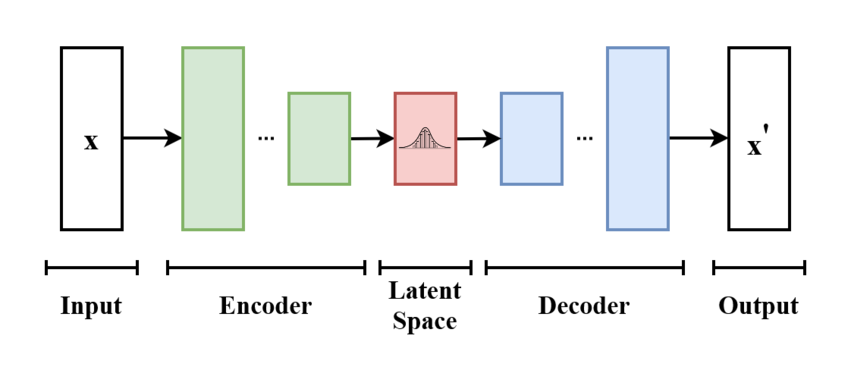
\includegraphics[width=\textwidth]{img/vaewiki.png}
        \caption{VAEs structure \textsuperscript{Source:wikipedia}}
        \label{fig:a}
    \end{subfigure}
    \hfill
        \begin{subfigure}{0.45\textwidth}
    \centering
        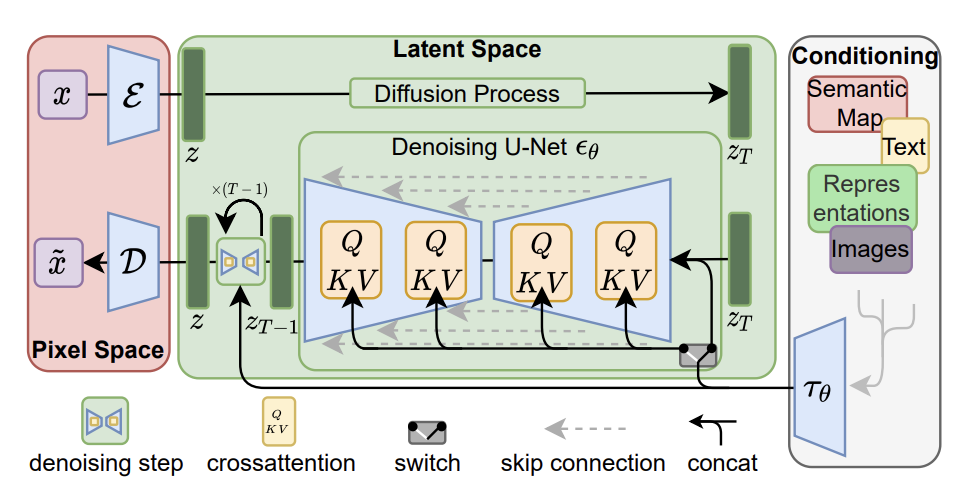
\includegraphics[width=\textwidth]{img/ldm.png}
        \caption{LDMs structure \textsuperscript{Source:\cite{rombach2022highresolutionimagesynthesislatent}}}
        \label{fig:c}
    \end{subfigure}

\end{figure}


\begin{figure}[htp]
    \centering
    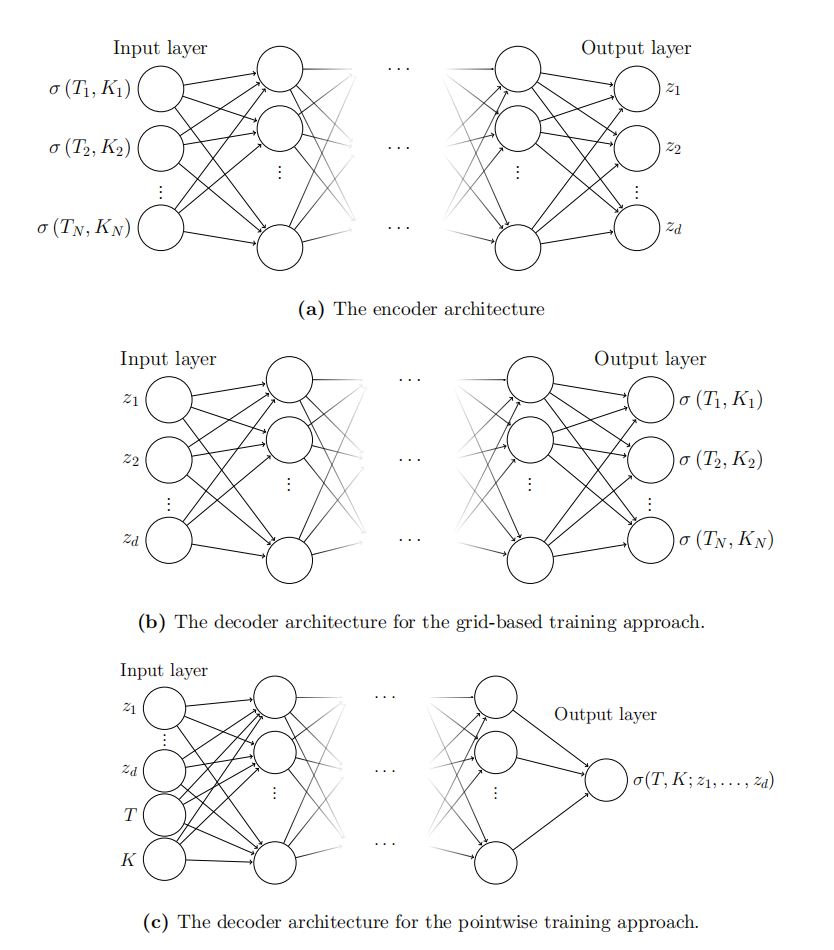
\includegraphics[width=0.6\linewidth]{img/vae_vol.png}
    \caption{Architectures of grid-based and pointwise method}
    \label{fig:b}
\end{figure}

\end{document}